\documentclass[a4paper, fontsize=12bp]{article}

\usepackage{scrextend}
\usepackage[T1]{fontenc}
\usepackage{mathtools}
\usepackage[utf8]{inputenc}
\usepackage[english, russian]{babel}
\usepackage{graphicx}
\usepackage{gensymb}
\usepackage{amssymb}
\usepackage{textcomp}
\usepackage{lastpage}
\usepackage{float}
\usepackage{afterpage}
\usepackage{titlesec}


\addtolength{\hoffset}{-1.75cm}
\addtolength{\textwidth}{3.5cm} 

\addtolength{\voffset}{-1.5cm}
\addtolength{\textheight}{3cm} 



\usepackage{fancyhdr}


%\titleformat{\section}[block]{\normalfont\sffamily}{\thesection}{.5em}%{\titlerule\\[.8ex]\bfseries}
%11111111111111111111111111111111111111111111111111111111111111111
\titleformat{\section}
    [block]{\normalfont\bfseries\large}{\rlap{\thesection}}{0em}
    {\vspace{-0.02\textwidth}\begin{minipage}[t]{.95\textwidth}}
[\end{minipage}]
%11111111111111111111111111111111111111111111111111111111111111111
\pagestyle{fancy}
	\fancyhf{}
	\lhead{\hspace{1bp} МФТИ, 2019}
	\rhead{Деревянкин Иван Б03-836 \hspace{1bp}}
	\cfoot{\textbf{ФАКИ}}
	\rfoot{\thepage\ \textnormal{из}\ \pageref{LastPage}}
	\renewcommand{\headrulewidth}{1.5bp}
	\renewcommand{\footrulewidth}{1.5bp}





%\titleformat{\section}
 %   [block]{\normalfont\bfseries\large}{\rlap{\thesection}}{0em}
 %   {\hspace{.05\linewidth}\begin{minipage}[t]{.95\textwidth}}
 %[\end{minipage}]


\begin{document}
\selectlanguage{russian}
\afterpage{
	\lhead{\hspace{10bp}  \textbf{Работа 2.2.1}}
	\rhead{\textit{Исследование взаимной диффузии газов} \hspace{10bp}}
	\cfoot{}
	\rfoot{\thepage\ \textnormal{из}\ \pageref{LastPage}}}




\huge
\centering
\textbf{Работа \textnumero2.2.1}


\Large
Исследование взаимной диффузии газов
\vspace{0.5cm}

\raggedright
\normalsize
\section*{Цель работы:}
1) Регистрация зависимости концентрации гелия в воздухе от времени с помощью датчиков теплопроводимости при разных начальных давлениях смеси газов;\\
2) Определение коэффициента диффузии по результатам измерений.

\section*{В работе используются:}
Измерительная установка; форвакуумный насос; баллон с газом (гелий); манометр; источник питания; магазин сопротивлений; гальванометр; секундомер.

\section*{{\large \textbf{Экспериментальная установка:}}}
\begin{figure}[H]
\center
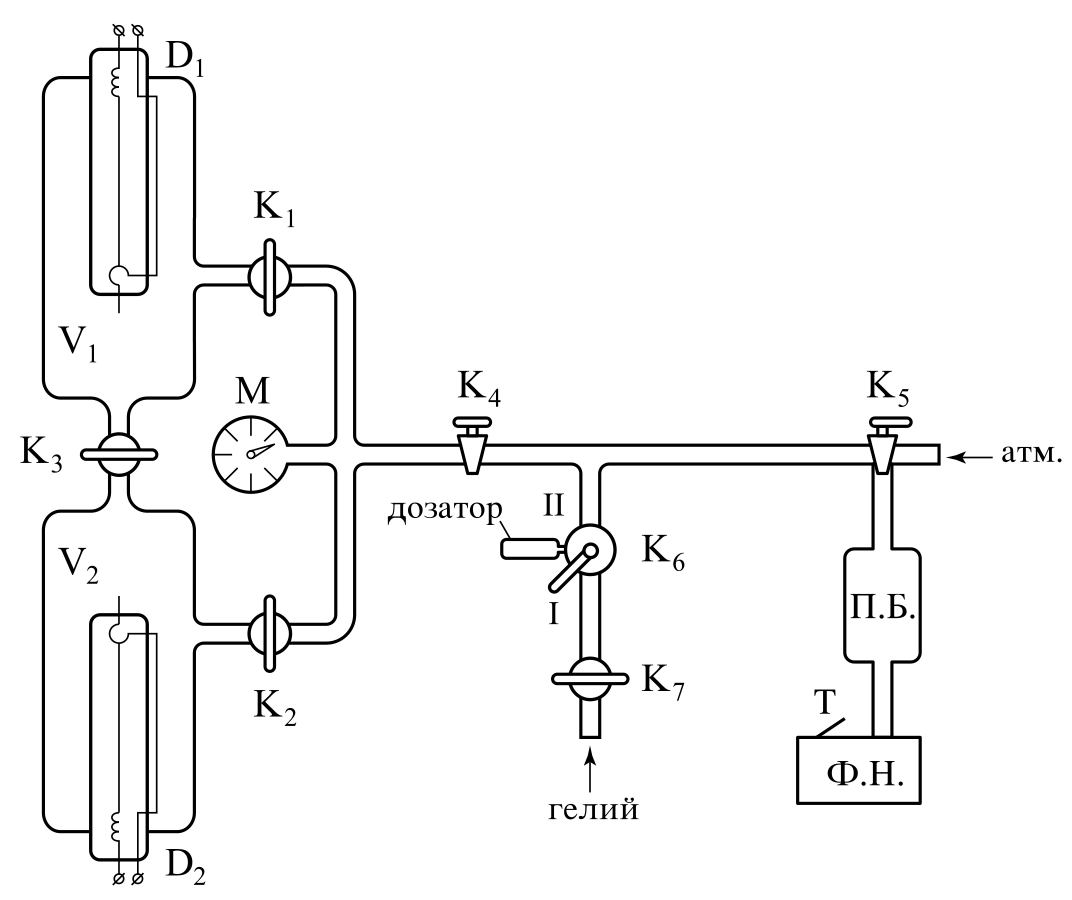
\includegraphics[scale=0.3]{asd.png}
\end{figure}
\section*{Теоретическая часть:}
Диффузией называется самопроизвольное перемешивание молекул, происходящее вследствие их теплового движения. В жидкости
диффузия происходит быстрее, чем в твердых телах, а в газах --- быстрее, чем в жидкостях. В тех случаях, когда изучается перемешивание молекул одного сорта, говорят о самодиффузии, а если перемешиваются разные молекулы --- о заимной (или концентрационной)
диффузии.

Рассмотрим процесс выравнивания концентрации. Пусть концентрации одного из компонентов смеси в сосудах $V_1$ и $V_2$ равны $n_1$ и
$n_2$ . Плотность диффузионного потока любого компонента (т. е. количество вещества, проходящее в единицу времени через единичную
поверхность) определяется законом Фика:
\[
j = - D \frac{\partial n}{\partial x},
\]
где $D$ --- коэффициент взаимной диффузии газов, а $j$ --- плотность
потока частиц. В наших условиях решение задачи упрощается благодаря тому, что: а) объем соединительной трубки мал по сравнению
с объемами сосудов, б) концентрацию газов внутри каждого сосуда
можно считать постоянной по всему объему. Диффузионный поток в
любом сечении трубки одинаков. Поэтому $J = - D S (\partial n / \partial x )$ не меняется вдоль трубки. Следовательно,
\[
	J = - D S \frac{n_1 - n_2}{l}.
\]
Обозначим через $\Delta n_1$ и $\Delta n_2$  изменения концентрации в объемах $V_1$ и $V_2$ за время $\Delta t$. Тогда $V_1 \delta n_1$ равно изменению количества компонента в объеме $V_1$, а $V_2 \Delta n_2$ --- изменению количества этого компонента в $V_2$. Из закона сохранения вещества следует, что $V_1 n_1 + V_2 n_2 = const$, откуда $V_1 \Delta n_1 = - V_2 \Delta n_2$. Эти изменения происходят вследствие диффузии, поэтому
\[
	V_1 \Delta n_1 = -V_2 \Delta n_2 = J \Delta t = -DS \frac{n_1 - n_2}{l} \Delta t.
\]
Деля это равенство на $\Delta t$, получим
\[
	V_1 \frac{dn_1}{dt} = -DS\frac{n_1 - n_2}{l}, \qquad V_1 \frac{dn_2}{dt} = DS\frac{n_1 - n_2}{l}.
\]
Разделив первое из этих уравнений на $V_1$, а второе на $V_2$ и вычтя эти равенства друг из друга, найдем
\[
	\frac{dn_1}{dt} - \frac{dn_2}{dt} = -\frac{n_1 - n_2}{l}DS \left( \frac{1}{V_1} - \frac{1}{V_2} \right).
\]
Введем новую переменную $n_1 - n_2$, после чего уравнение легко интегрируется:
\begin{equation}
\label{1}
	n_1 - n_2 = {(n_1 - n_2)}_0e^{-t/\tau},
\end{equation}
где ${(n_1 - n_2)}_0$ --- разность концентраций в начальный момент времени,
\begin{equation}
	\tau = \frac{V_1 V_2}{V_1 + V_2}\frac{l}{SD}
\end{equation}
Формула (\ref{1}) показывает, что разность концентраций убывает по экспоненциальному закону, и тем быстрее, чем меньше $\tau$ (постоянная
времени процесса). Величина $\tau$ определяется геометрическими разме-
рами установки $(l, S, V_1, V_2)$ и величиной коэффициента диффузии
$D$. Для измерения концентраций в данной установке применяются
датчики теплопроводности $D_1$ , $D_2$ и используется зависимость 
теплопроводности газовой смеси от ее состава. Тонкая проволочка радиуса 
$r_{\text{пр}}$, протянутая вдоль оси стеклянного цилиндра радиуса 
$R_{\text{ц}}$, нагревается током. Тепло от проволочки к стенке цилиндра
переходит главным образом вследствие теплопроводности газа, находящегося 
внутри цилиндра. Количество тепла, передающееся стенке
в единицу времени:
\[
	Q = \varkappa\frac{2\pi L}{\ln(R_{\text{ц}} / r_{\text{пр}} )}\left(T_1 - T_2 \right),
\]
где $\varkappa$ --- теплопроводность, $L$ --- длина нити, $T_1$, $T_2$ --- 
температуры проволочки и стенки. При заданном режиме нагревания $(Q = const)
$ температура проволочки и соответственно ее сопротивление определяются 
теплопроводностью газа и, следовательно, его составом. В процессе диффузии 
разность концентраций убывает по закону (\ref{1}). Потому же закону изменяются во времени показания гальванометра (например, в делениях шкалы), т. е.
\[
	N = N_0e^{-t/\tau},
\]
где $N_0$ --- показание в начальный момент времени.
\section*{Обработка результатов измерений:}
Геометрические параметры установки:
\\
\begin{figure}[H]
\center
\begin{tabular}{|c|c|c|c|c|}
\hline $V_1, \text{см}^3$, & $V_2, \text{см}^3$ & $L/S, 1/\text{см}$ &
$P_{\text{гел}}$ & $P_{\text{воз}}$ \\
\hline $420 \pm 10$ & $420 \pm 10$ & $9.0 \pm 0.1$ & $0.2 P_{\text{раб}}$
	& $1.7 P_{\text{раб}}$ \\ \hline
	\end{tabular}
\end{figure}
\begin{figure}[H]
\begin{minipage}[h]{0.47\linewidth}
\center{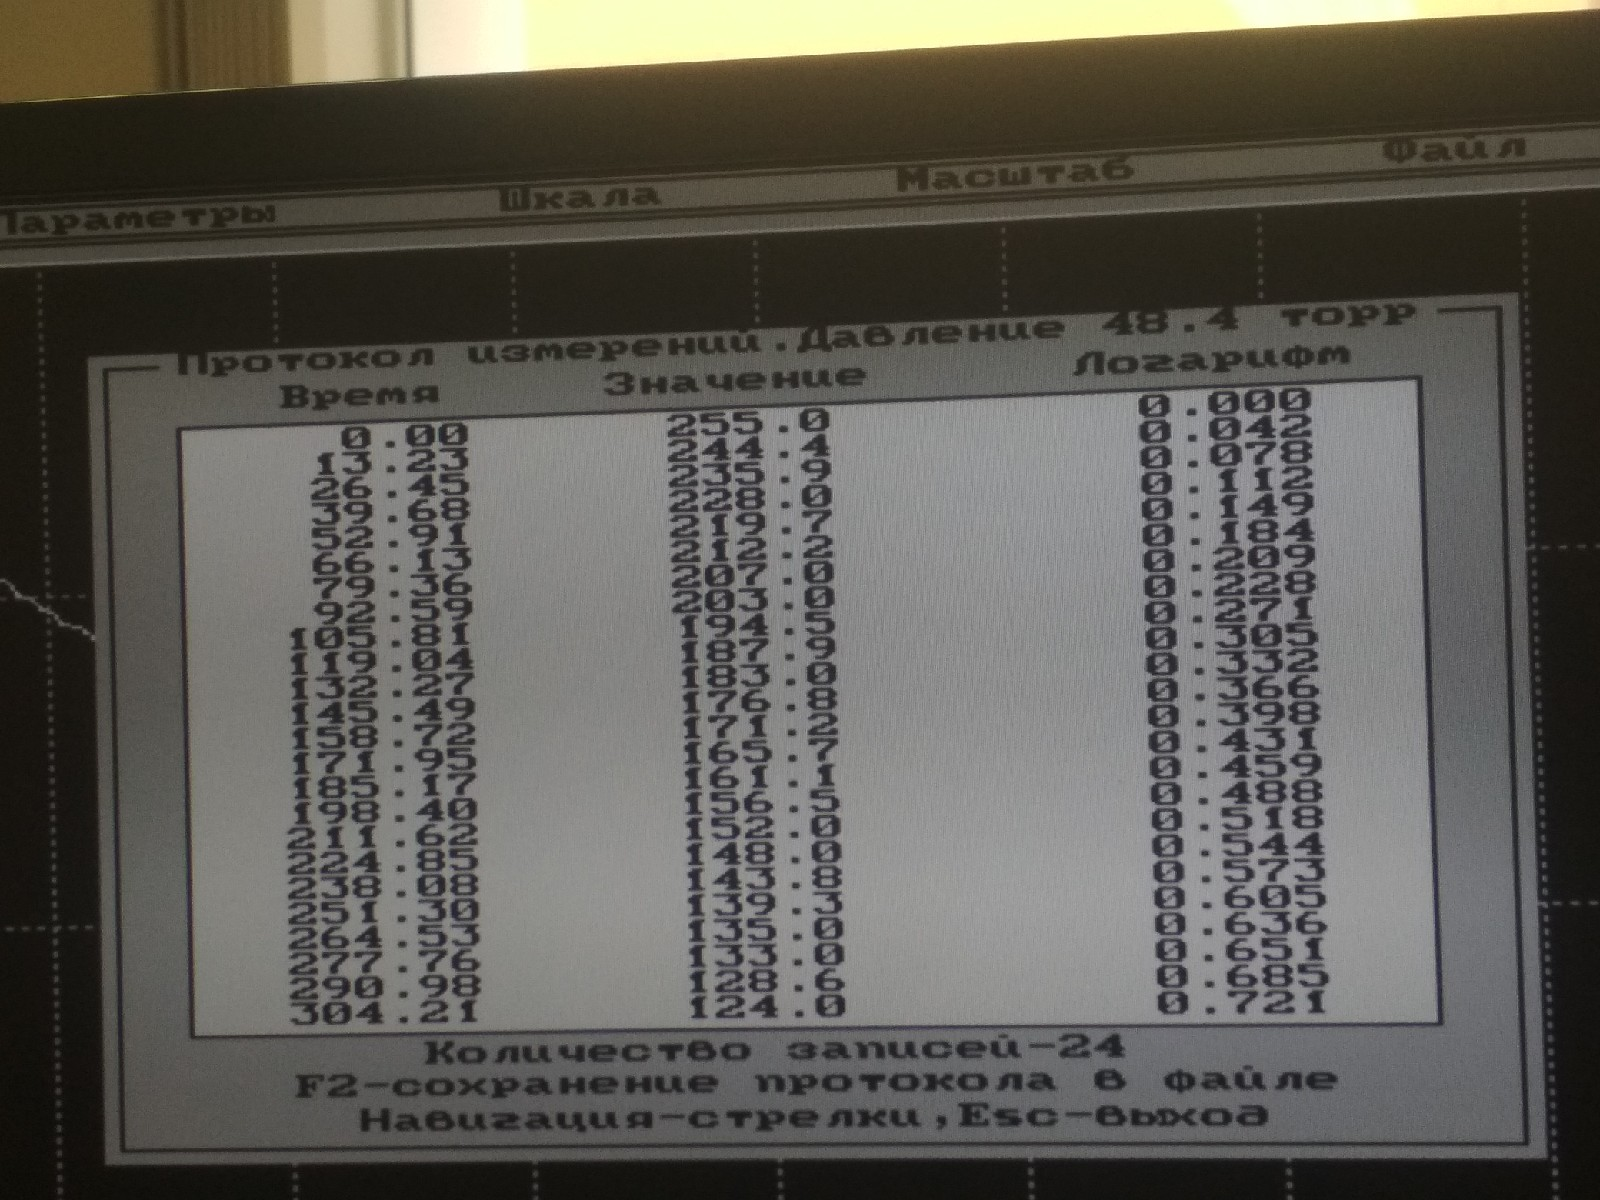
\includegraphics[width=1\linewidth]{40.jpg}} а) 48.4 Торр \\
\end{minipage}
\hfill
\begin{minipage}[h]{0.47\linewidth}
\center{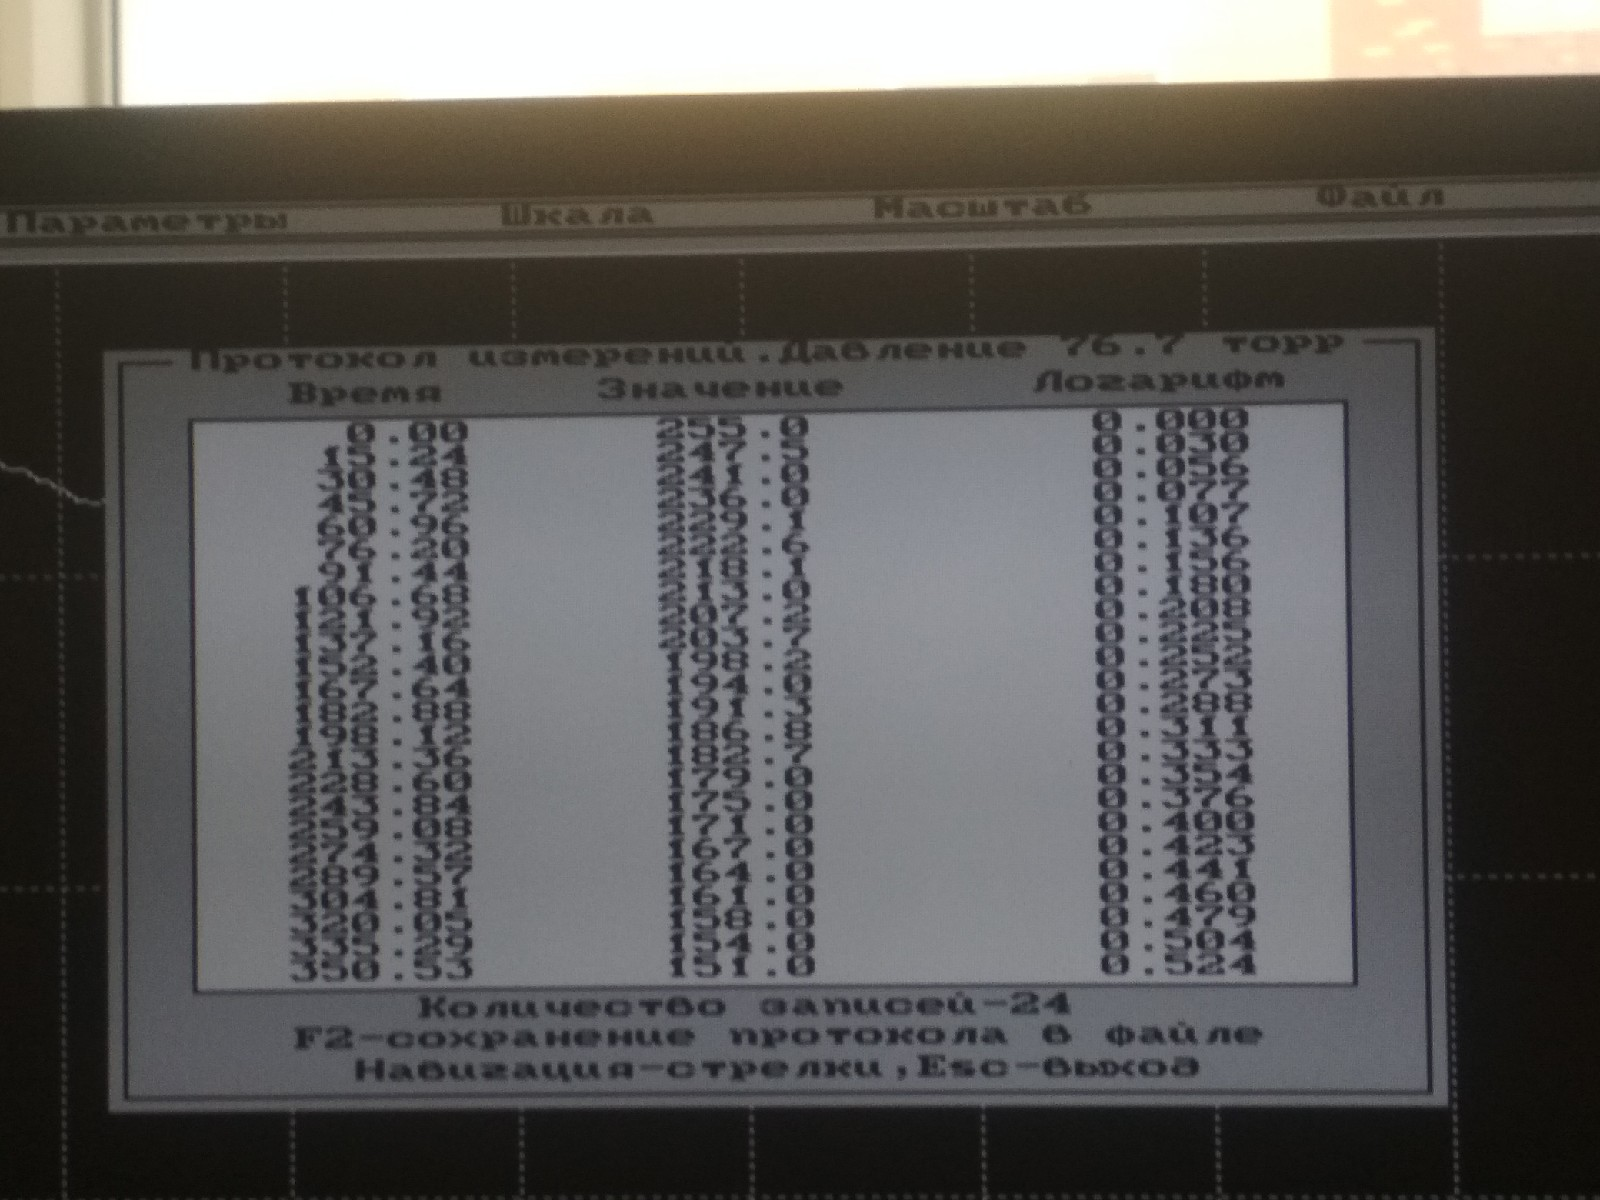
\includegraphics[width=1\linewidth]{75.jpg}} \\б) 76.7 Торр
\end{minipage}
\vfill
\begin{minipage}[h]{0.47\linewidth}
\center{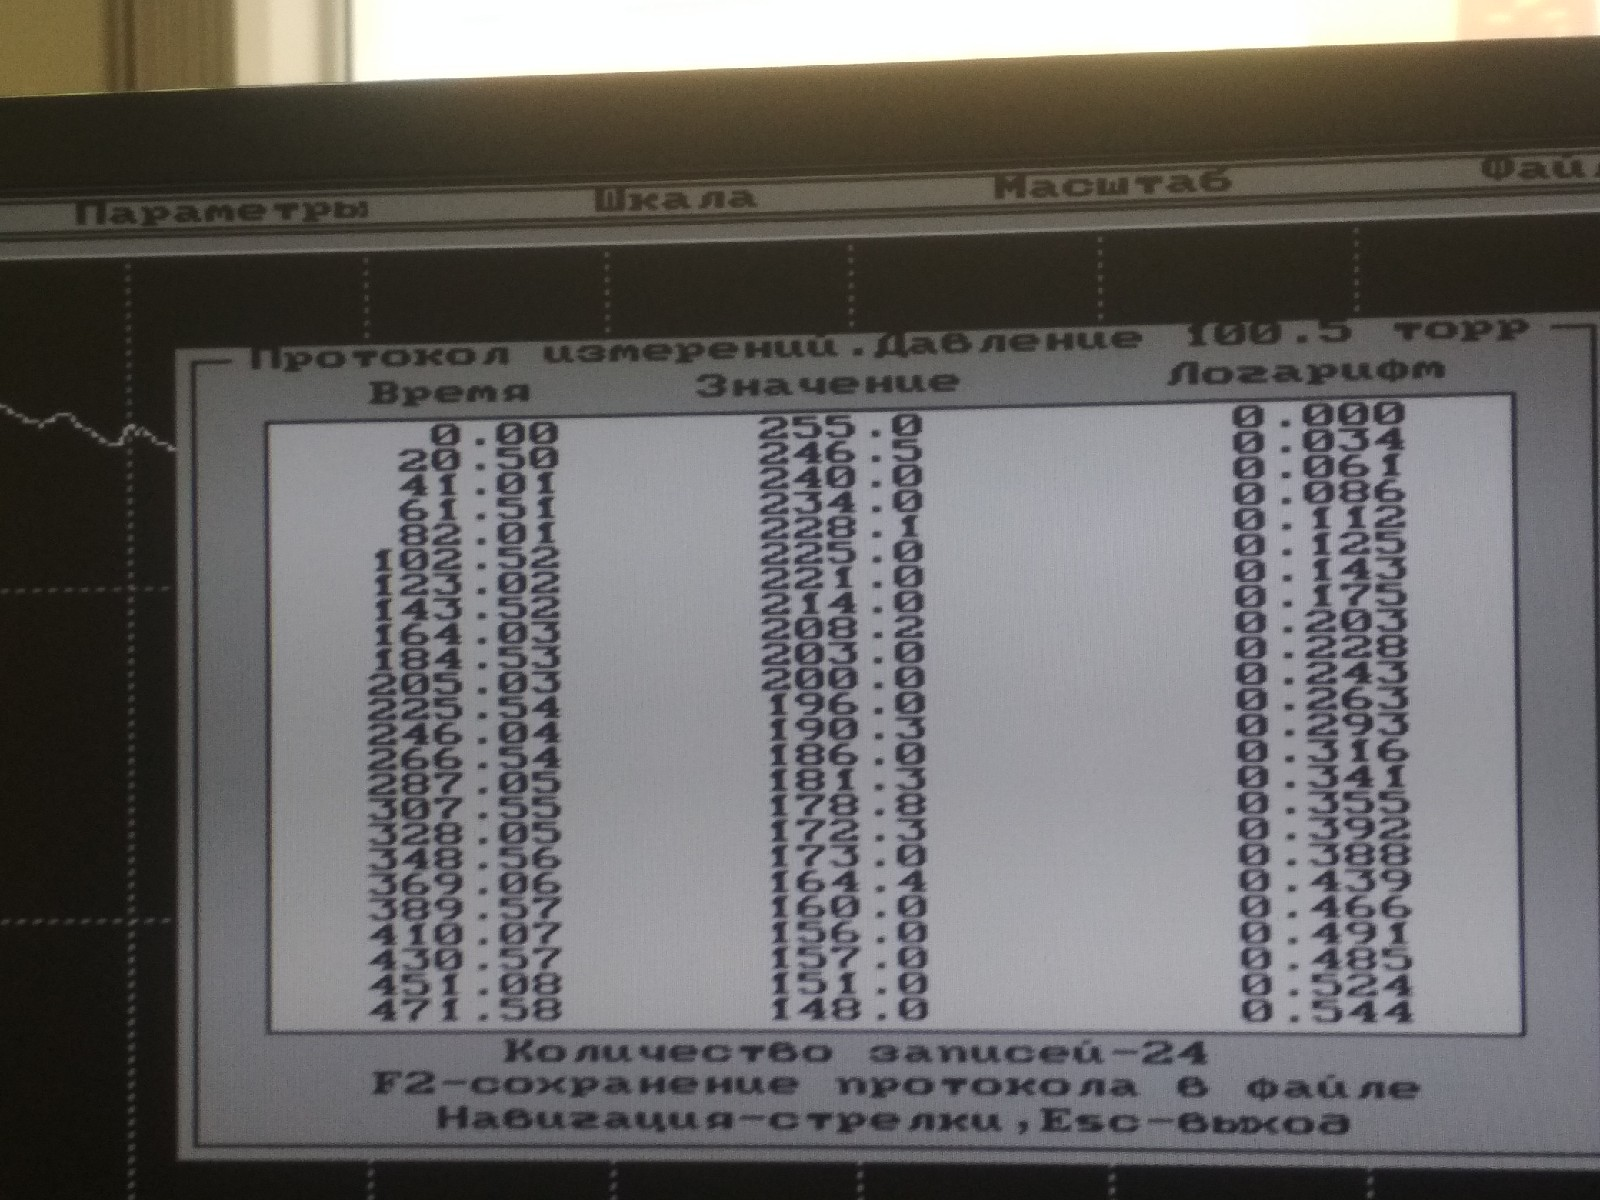
\includegraphics[width=1\linewidth]{100.jpg}} в) 100.5 Торр \\
\end{minipage}
\hfill
\begin{minipage}[h]{0.47\linewidth}
\center{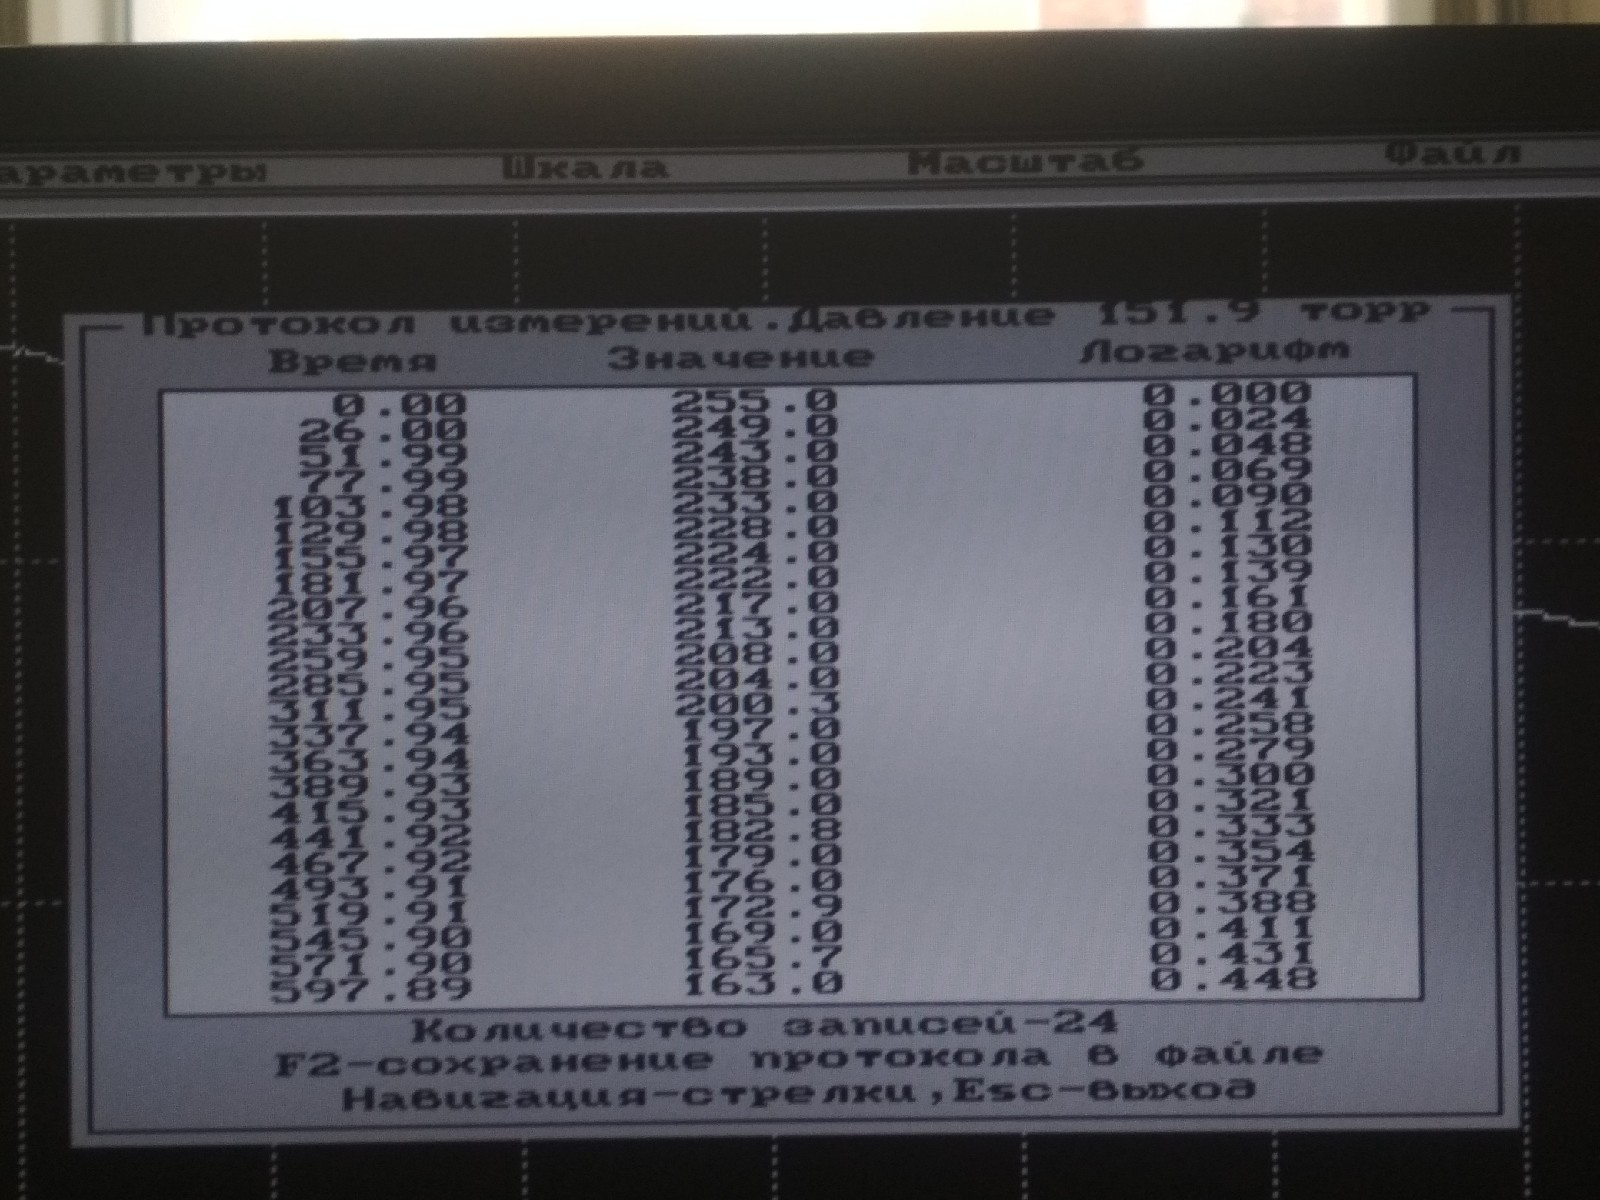
\includegraphics[width=1\linewidth]{150.jpg}} г) 151.9 Торр \\
\end{minipage}
\caption{Измерения при давлении $P_{\text{рабочее}}$}
\end{figure}

Для каждого из давлений построим графики, откладывая по оси абсцисс время, а по оси ординат --- логарифм от показаний гальванометра и находём угловые коэффициенты каждой прямой:
\begin{figure}[H]
\begin{minipage}[h]{0.47\linewidth}
\center{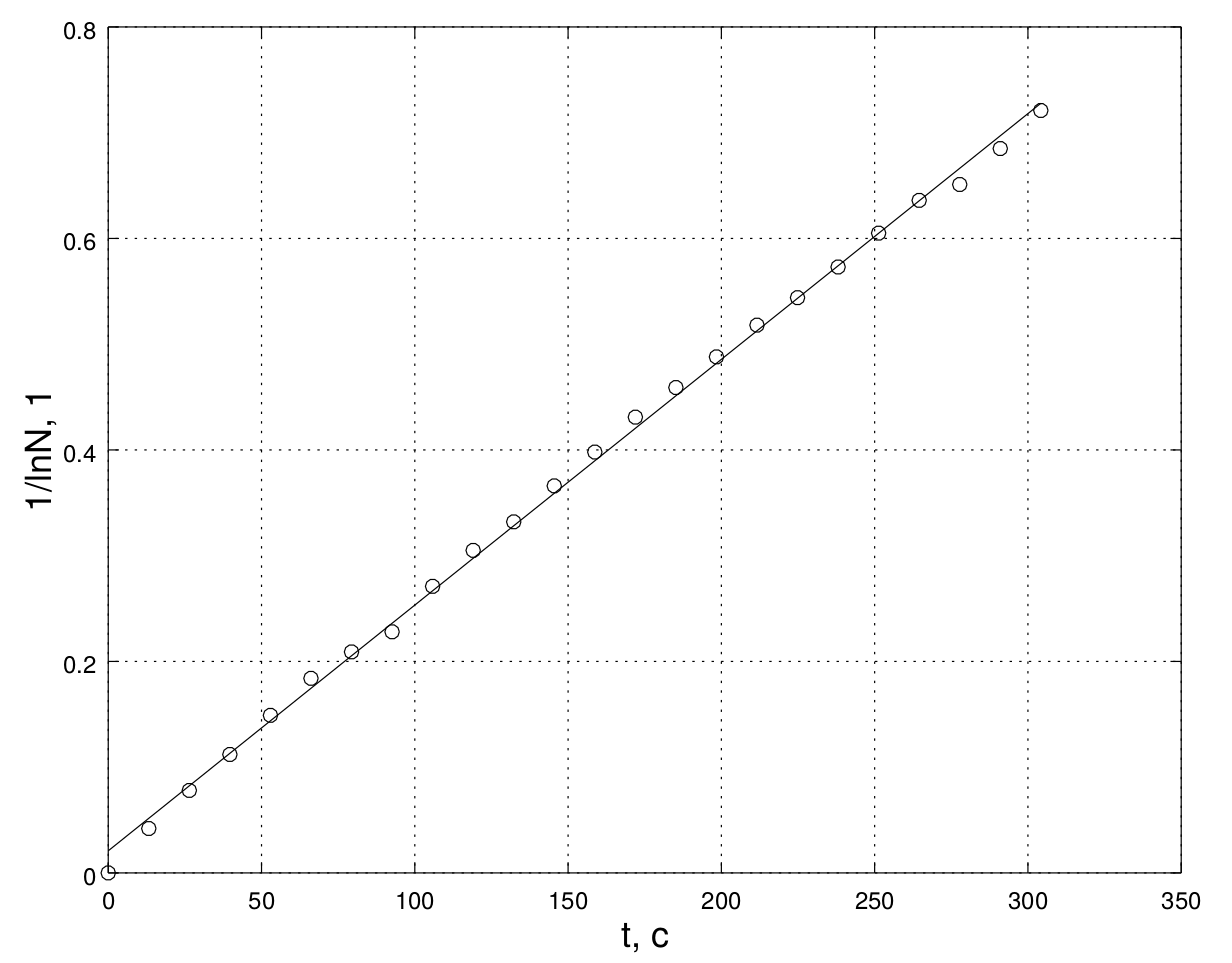
\includegraphics[width=1\linewidth]{40g.png}} а) 48.4 Торр \\
\end{minipage}
\hfill
\begin{minipage}[h]{0.47\linewidth}
\center{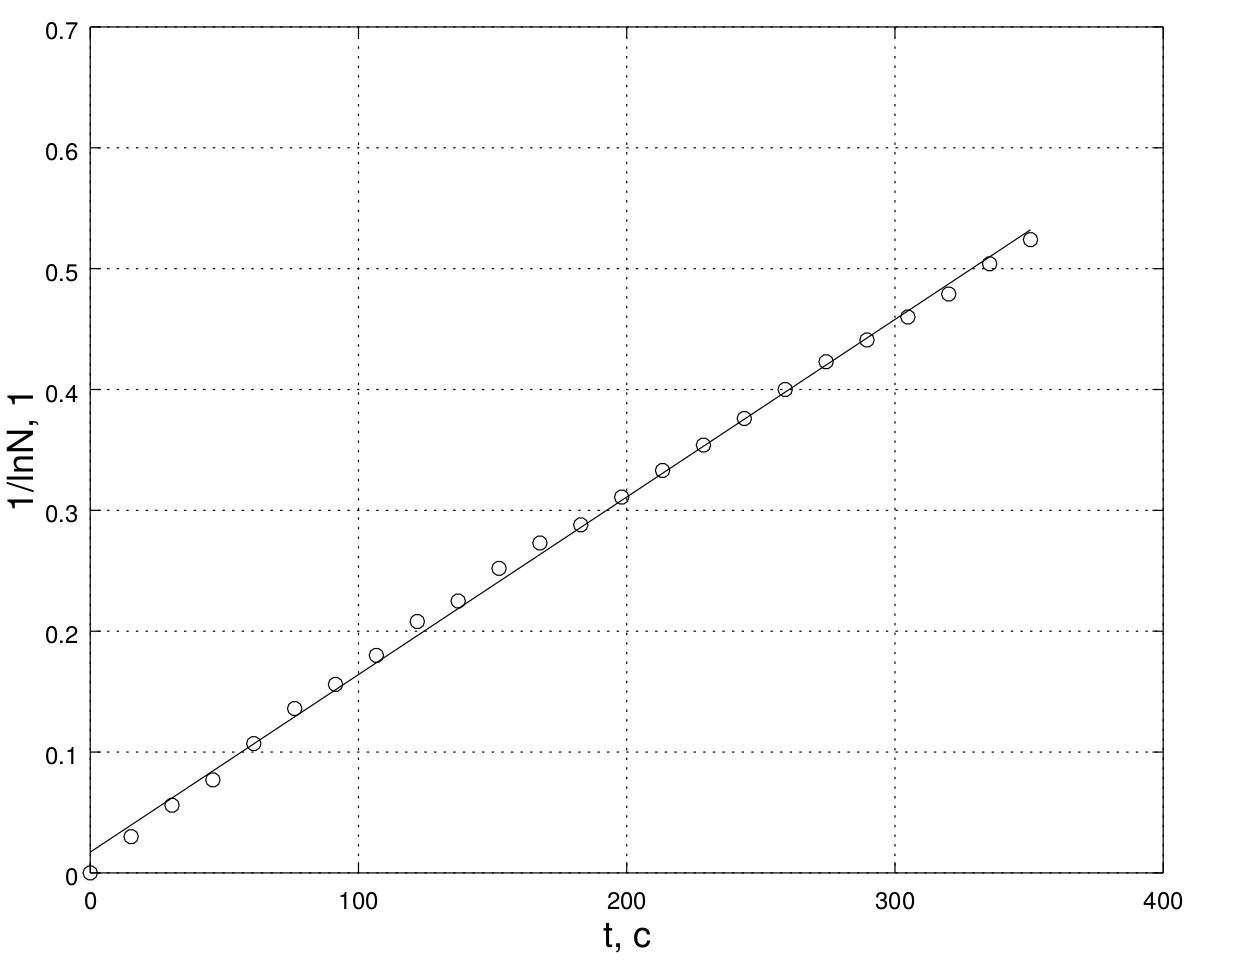
\includegraphics[width=1\linewidth]{75g.png}} \\б) 76.7 Торр
\end{minipage}
\vfill
\begin{minipage}[h]{0.47\linewidth}
\center{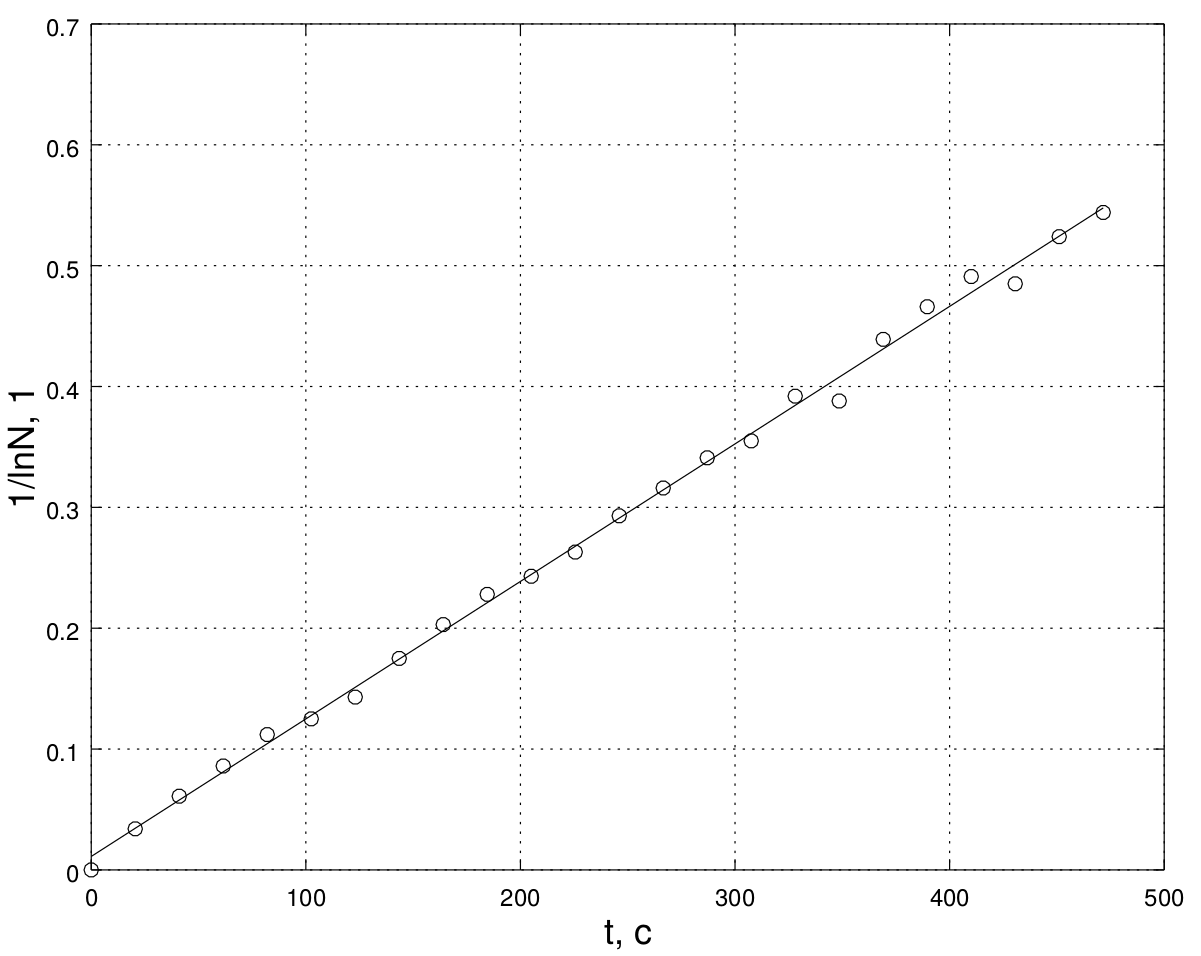
\includegraphics[width=1\linewidth]{100g.png}} в) 100.5 Торр \\
\end{minipage}
\hfill
\begin{minipage}[h]{0.47\linewidth}
\center{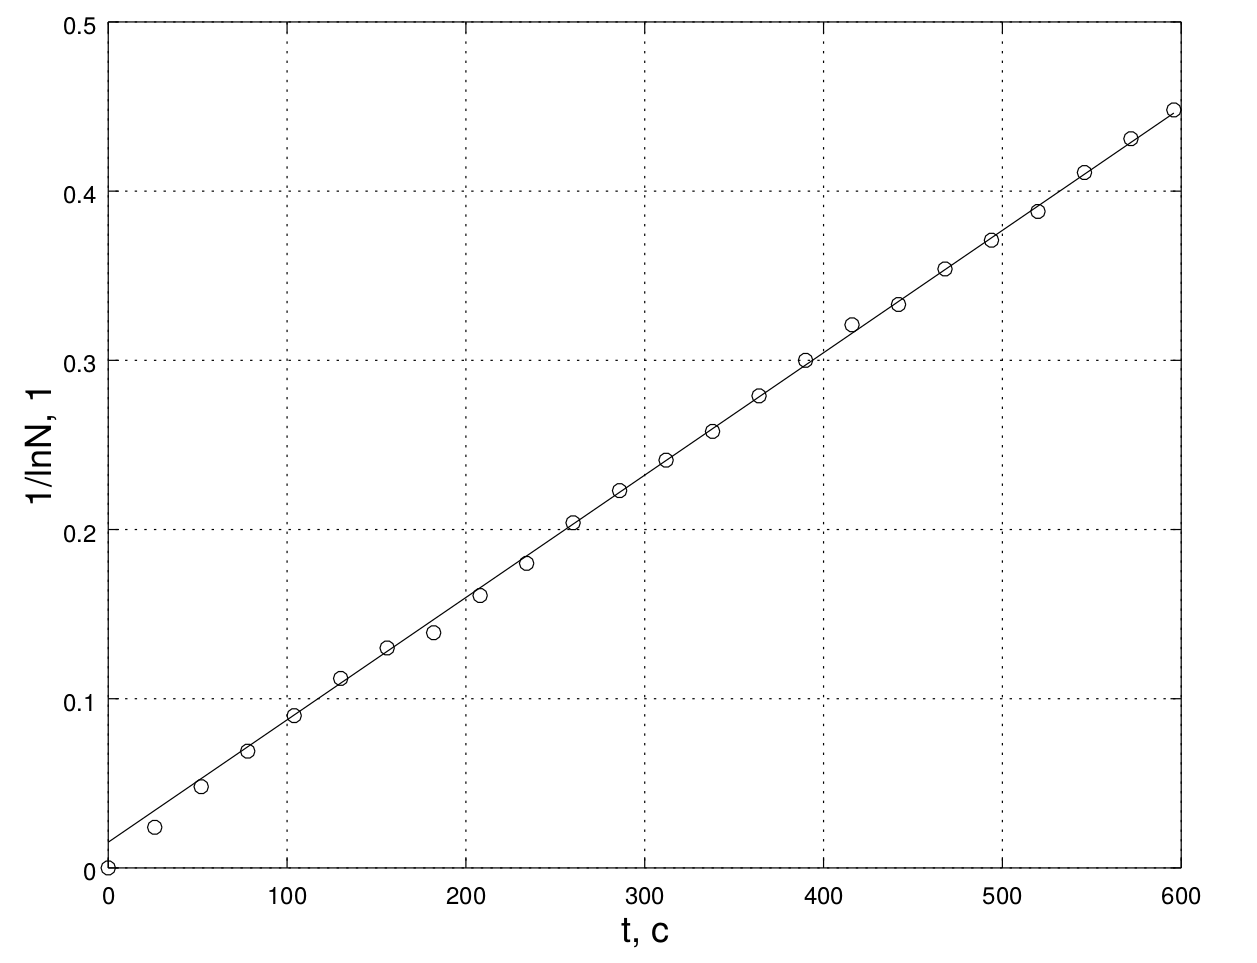
\includegraphics[width=1\linewidth]{150g.png}} г) 151.9 Торр \\
\end{minipage}
\caption{Графики в координатах $\ln\! N(t)$ при давлениях $P_{\text{рабочее}}$}
\end{figure}
Угловые коэффициенты графиков:
\begin{figure}[H]
\center
\begin{tabular}{|c|c|c|c|}
\hline $1/\tau_1,\ 10^{-3} 1/c$ & $1/\tau_2,\ 10^{-3} 1/c$ & $1/\tau_3,\  10^{-3} 1/c$ & $1/\tau_4,\ 10^{-3} 1/c$ \\
\hline $2.33 \pm 0.05$ & $1.47 \pm 0.03$ & $1.14 \pm 0.03$ &  $0.74 \pm 0.02$\\\hline
	\end{tabular}
\end{figure}
\section{Обработка результатов измерений:}
 Найдём коэффициенты взаимной диффузии газов при выбранных давлениях из формулы (2):
 \[
  D=\frac{L}{S} \cdot \frac{V_1V_2}{V_1+V_2} \cdot \frac{1}{\tau}
  \]
\\
\begin{figure}[H]
\center
\begin{tabular}{|c|c|c|c|}
\hline $D_1,\ \frac{\text{см}^2}{c}$ & $D_2,\ \frac{\text{см}^2}{c}$ & $D_3,\ \frac{\text{см}^2}{c}$ & $D_4,\ \frac{\text{см}^2}{c}$ \\
\hline $4404 \pm 202$ & $2778 \pm 139$ & $2155 \pm 108$ &  $1399 \pm 70$\\\hline
	\end{tabular}
\end{figure}
Построим график зависимости $D(\frac{1}{P})$ и по его коэффициенту наклона рассчитаем величину коэффициента диффузии при атмосферном давлении:
\begin{figure}[H]
\center
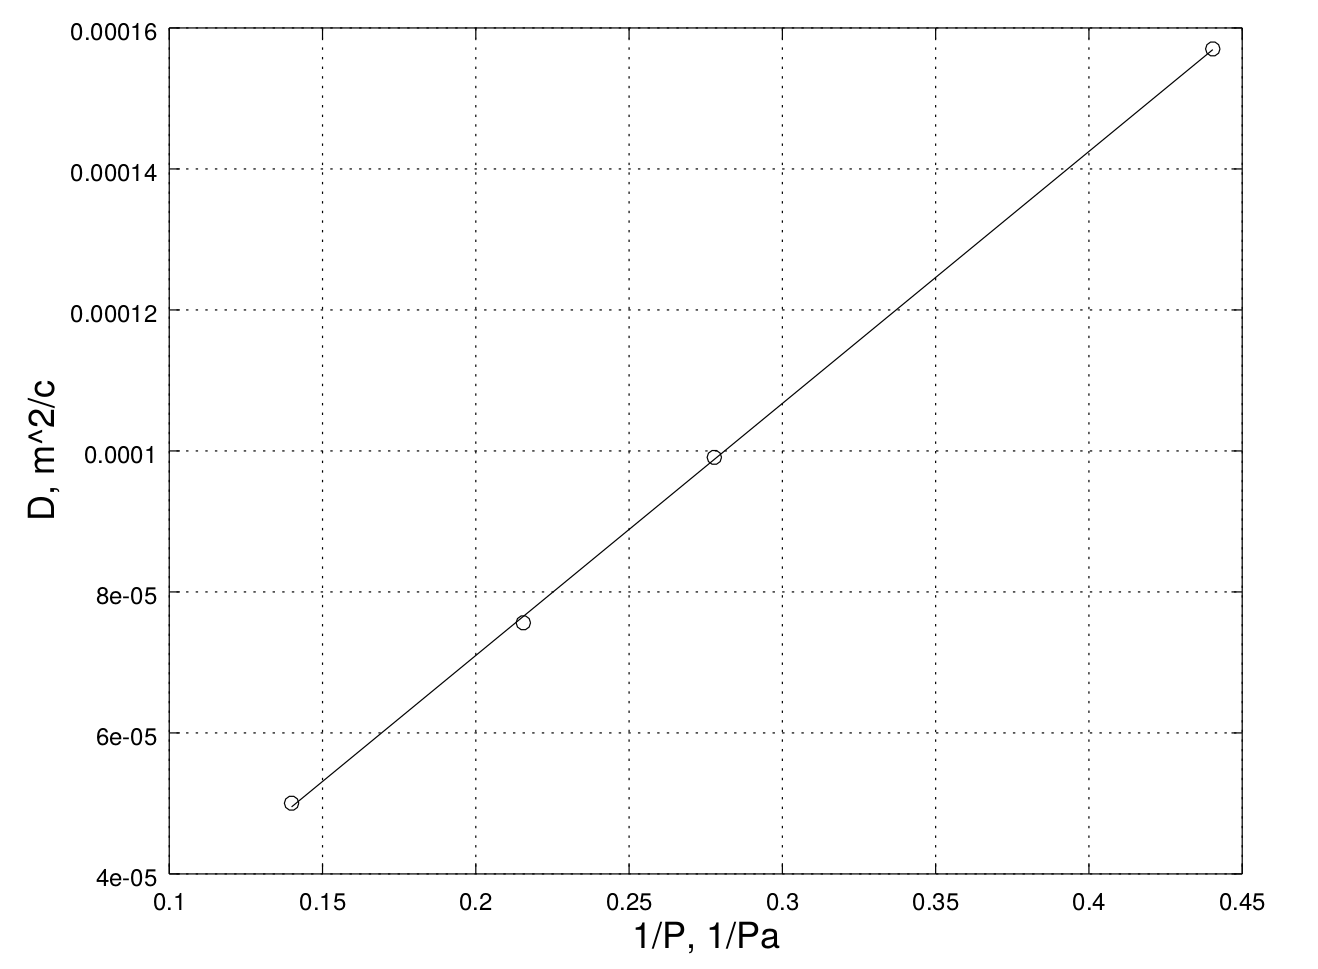
\includegraphics[scale=0.2]{dp.png}
\caption{График зависимости $D(\frac{1}{P})$}
\end{figure}
Коэффициент наклона графика $K = (3.575 \pm 0.14) \cdot 10^{-4}$
Для $T = 293 K$ и $P = 760\ \text{мм.\ рт.\ ст.} \approx 10^5\ \text{Па}$ найдем диффузии при нормальных условиях из графика:
$D(\frac{1}{P})$:
\[
	D = (0.54 \pm 0.06) \cdot 10^{-4}\ \frac{\text{м}^2}{c}
\]
\section*{Вывод:}
В данной работе мы зарегистрировали зависимости концентрации гелия в воздухе от времени с помощью датчиков теплопроводимости при разных начальных давлениях смеси газов и нашли коэффициент взаимной диффузии газов при нормальных условиях.
\end{document}